% Chapter 4

\chapter{SYSTEM ARCHITECTURE} \label{ch4}
This chapter describes the overall architecture of the project. The first section(\ref{ch4Env}) covers the custom environment that we have developed using Unity game Engine for conducting our experiment. We then describe our the agent(\ref{ch4Agent}) wherein the agent, the methods by which the agent perceives the environment (\ref{ch4inp}), obtains the rewards and takes decisions using the PPO algorithm are discussed . The penultimate section(\ref{ch4TL}) introduces the Transfer Learning process by which the knowledge learnt by the agent in one track is transferred to another track in our environment. Finally, we cover adversarial attacks(\ref{ch4AT}) on the action space and the observation space of the agent and performing Transfer Learning using Adversarial Training as a precursor.

\section{ENVIRONMENT} \label{ch4Env}



To perform Deep Reinforcement learning we have designed and created our own custom environment in Unity game engine. We have used a package called MLagents developed specifically for Unity that allows us to run our reinforcement learning algorithms in the environment.

We have designed 5 tracks of varying complexity to measure model performance in environments having the same action space. We shall further explore the different tracks in the upcoming chapters. 

Building the environment from scratch, allows us to have greater control over the different events that may occur and influence the agent. All the environments have similar events that are used to return a scalar reward to the agent.



The tracks are built using 4 major components : the sidewall(3), the checkpoints(2), the agent(1) and the ray perception sensors(4) as seen in figure \ref{fig:agent-inputs}

There are numerous checkpoints along the tracks that are placed approximately equidistant to one another. These checkpoints are used to encourage the agent to go in the right direction, and to measure how far the agent has progressed in a track. These invisible checkpoints have an event associated with them that enables the agent to detect them when a collision occurs. When this event is fired, we check if the current checkpoint is the correct checkpoint or not and appropriately provide a reward.

The sidewalls are solid game objects that are used to make sure the agent/car doesn't veer off track. When the agent collides with the sidewall, a function is triggered and a negative reward is sent to the agent. The ray-perception sensors are sensory beams originating from the car/agent, that allow the agent to detect the other game objects and components in the environment. The interactions between these 4 core components enable us to set our scalar rewards, that guide the agent and provide the essential logic required for training.


\subsection{REWARD SCHEME}

The reward scheme is crucial to enable the agent to train for the task. Rewards need to be provided at a constant interval when the agent is performing as expected in order to train faster and similarly negative rewards need to be provided immediately when performance is unexpected in order to train the agent faster. By experimenting with various permutations, we have arrived at the following reward scheme for the agent:

\begin{enumerate}
    \item \textbf{At each step}: A \textit{small negative} reward is provided to incentivize the agent to travel quicker around the track.
    \item \textbf{OnWallCollision:} A \textit{moderate negative} reward is provided to discourage agent from hitting the walls on the track.
    \item \textbf{OnWallCollisionStay:} The difference between collision stay and collision is that once an object has collided in Unity, if it is still in contact with the object post collision, a separate event called OnCollisionStay is triggered and hence a \textit{small negative} reward is provided to prohibit agent from using the walls to perform its turning actions.
    \item \textbf{CorrectCheckpoint:} The car has managed to make some progress in the track and hence to reward its progress, a \textit{positive} reward is provided.
    \item \textbf{IncorrectCheckpoint:} The car is moving in the wrong direction on the track and hence to prevent it from continuing to do so, we provide a \textit{negative} reward when it passes through an incorrect checkpoint.
    \item \textbf{LapCompleted:} The car has completed a lap successfully around the track and hence a \textit{large positive} reward is provided to the agent.
\end{enumerate}


\section{AGENT} \label{ch4Agent}

\subsection{Actor-Critic Methods}
Actor Critic Methods are a subclass of Reinforcement Learning algorithms. They consist of a “Critic” and an “Actor” entities during the training process. The “Critic” estimates the value function, ie, the value or predicted reward of a given state. This value function could be a state or action value function. The “Actor” in turn, makes use of the Critic’s output in order to update the policy distribution, and takes action based on the current policy. The samples generated by the Actor in turn, are used to update the value estimates of the Critic. Both the Actor and Critic are function approximators, generally with neural networks. 

\begin{figure}[H]
    \centering
    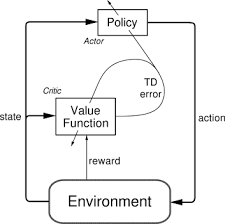
\includegraphics[width=0.45\textwidth]{images/ActorCriticMethod.png}
    \caption{Actor Critic Methods}
    \label{fig:rl}
\end{figure}

\subsection{Proximal Policy Optimization}
Proximal Policy Optimization (PPO) is an RL algorithm that falls under the actor-critic class of methods. It is a policy gradient method, ie, it uses a function approximator to represent the policy and performs gradient ascent on it to obtain the maximum reward. The main advantage of PPO over vanilla policy gradient or actor-critic algorithms is the fact that PPO clips the updates made to its value function to a certain extent. By clipping its updates, PPO ensures that the policy doesn’t go too far in the wrong direction and ruin its chances of finding the optimal solution.

In order to understand how PPO performs this clipping, we need to understand a few key terms first. The first term is $r(\theta)$. $r(\theta)$ is defined as the probability ratio of an action under the current policy and the action under the previous policy. If a particular action becomes more likely to be taken by the current policy, the value of $r(\theta)$ will be greater than 1. If a particular action becomes less likely to be taken by the current policy, the value of $r(\theta)$ will be between 0 and 1.

% \begin{figure}[H]
%     \centering
%     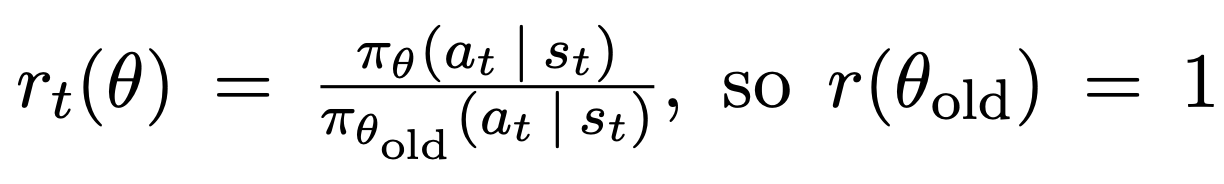
\includegraphics[width=0.75\textwidth]{images/r-theta.png}
%     \caption{r(theta)}
%     \label{fig:rl}
% \end{figure}


\begin{equation}
    r_{t}(\theta) = \frac{\pi_{\theta}(a_{t}|s_{t})}{\pi_{\theta}_{old}(a_{t}|s_{t})}, so\; r(\theta_{old}) = 1
\end{equation}


The second term is the advantage $\hat{A}_{t}$. The advantage $\hat{A}_{t}$ is an estimate of the relative value of the selected action in the current state. This advantage is used to estimate how good a particular action is compared to the average action in that state. The advantage is used to reduce variance in the updates made to the value function. If the advantage function for an action is positive, it means that action is good and will generate better rewards in the future. Therefore, we should increase the probability of picking that particular action in the future. On the other hand, if the advantage function for an action is negative, the probability of picking that action should be reduced.

% \begin{figure}[H]
%     \centering
%     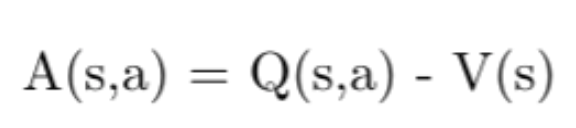
\includegraphics[width=0.75\textwidth]{images/advantage-function.png}
%     \caption{Advantage Function}
%     \label{fig:rl}
% \end{figure}
\begin{equation}
    A(s,a) = Q(s,a) - V(s)
\end{equation}
The general method in which policy-gradient methods work is by optimizing a policy loss function. Optimizing this function for reward can theoretically lead to an optimized function, but it is often quite difficult due to the nature of the samples. During the training process, the neural network representing our value function is constantly being updated, therefore our values are quite noisy and may not be very accurate.

PPO aims to solve this issue by making use of both of these terms, ie, $r(\theta)$ and $\hat{A}_{t}$, to generate a unique loss function called the Clipped Surrogate Objective. Clipped Surrogate Objective computes the minimum of two terms: the normal PG(Policy gradient) objective and clipped PG objective. The key component in PPO is the 2nd term, which clips the normal PG objective between $1 + \epsilon$ and $1 - \epsilon$. The effects of this clipping can be captured in the below graphs. 

% \begin{figure}[H]
%     \centering
%     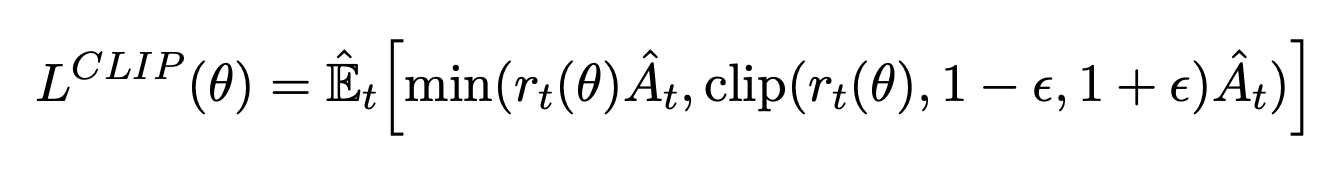
\includegraphics[width=0.75\textwidth]{images/clip-ppo.png}
%     \caption{Clipped Loss}
%     \label{fig:rl}
% \end{figure}

\begin{equation}
    L^{CLIP}(\theta) = \hat{\mathbb{E}}_{t}[min(r_{t}(\theta) \hat{A}_{t}, clip(r_{t}(\theta), 1- \epsilon, 1 + \epsilon)\hat{A}_{t})]
\end{equation}

\begin{figure}[H]
    \centering
    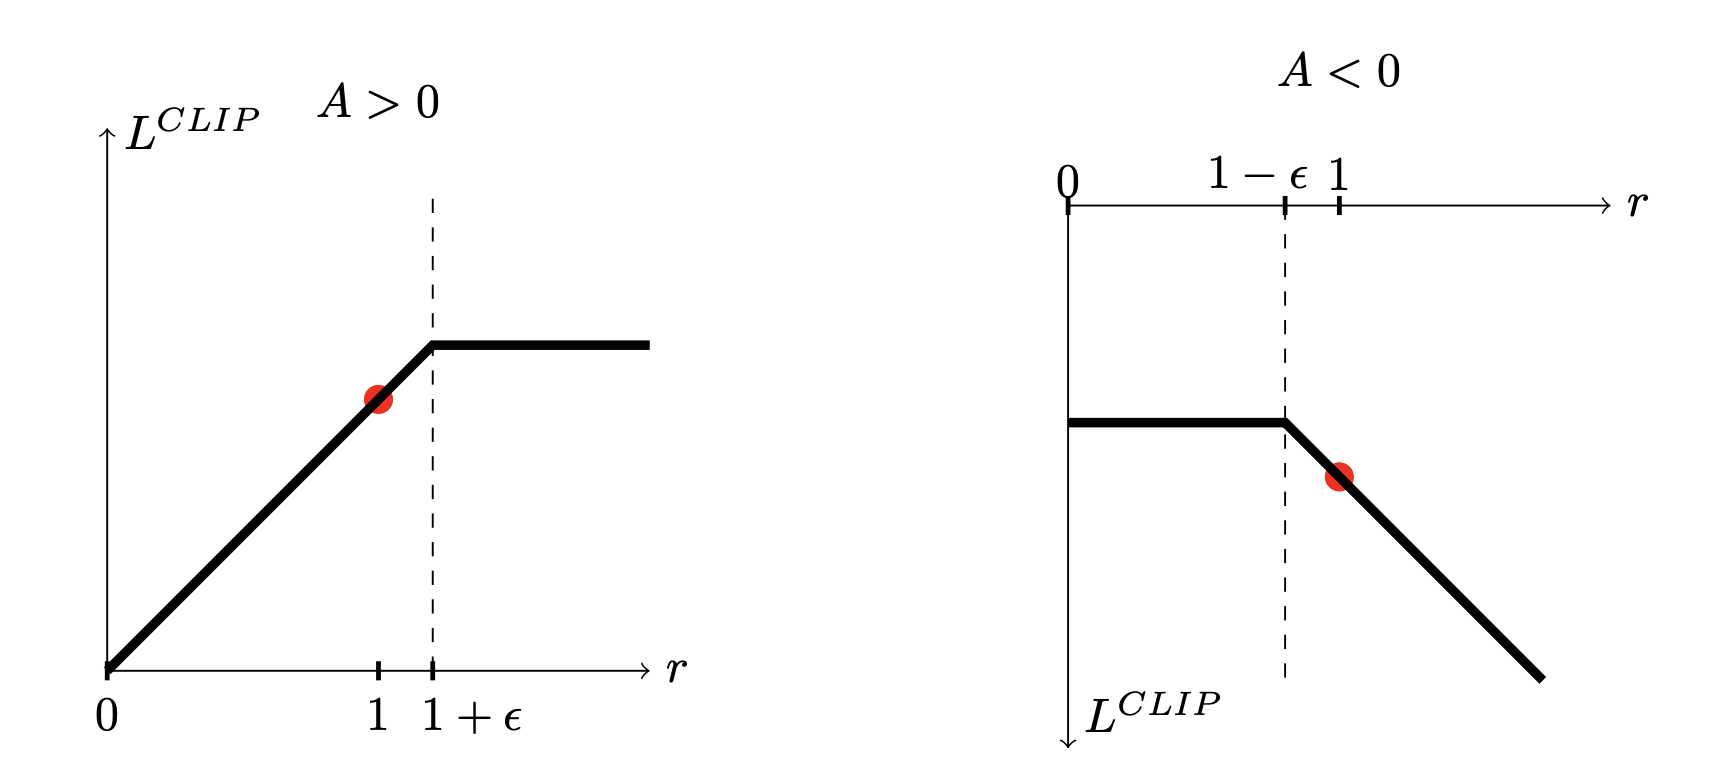
\includegraphics[width=0.75\textwidth]{images/clipped-loss-graph.png}
    \caption{Clipped Loss Graph}
    \label{fig:rl}
\end{figure}


On the left side, we see the scenario where the advantage is positive, i.e., the action taken by the agent had a better-than-expected return. With increasing values of r, the value of the $L^{CLIP}$ also increases, but only to a certain point. This prevents the algorithm from taking an update too far in the wrong direction. A similar scenario takes place on the right side as well. The algorithm is prevented from over-correcting its mistakes. 

PPO combines this loss function with two other terms, namely $L^{VF}$ and $S$. $L^{VF}$ is the mean squared error of the value function that is in charge of updating the network. S is a measure of entropy, which helps the agent act spontaneously in the initial stages of training, which can help the agent experiment and find optimal actions.



% \begin{figure}[H]
%     \centering
%     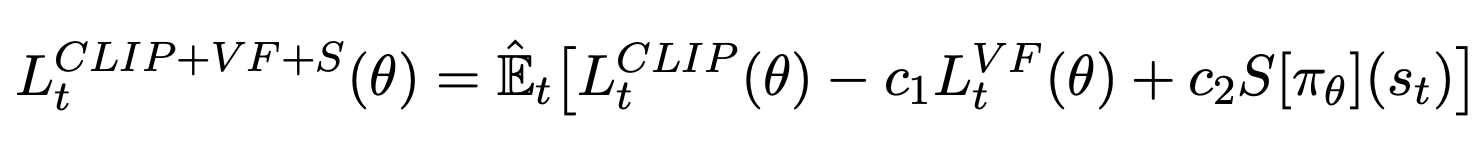
\includegraphics[width=0.75\textwidth]{images/ppo-final-loss.png}
%     \caption{Final Loss}
%     \label{fig:rl}
% \end{figure}

\begin{equation}
    L_{t}^{CLIP+VF+S}(\theta) = \hat{\mathbb{E}}[L_{t}^{CLIP}(\theta) - c_{1}L_{t}^{VF}(\theta) + c_{2}S[\pi_{\theta}](s_{t})] 
\end{equation}

% \section{ALGORITHM: PPO} \label{ch4-ppo-alg}



\subsection{ALGORITHM: PPO} \label{ch4-ppo-alg}

% \begin{figure}[H]
%     \centering
%     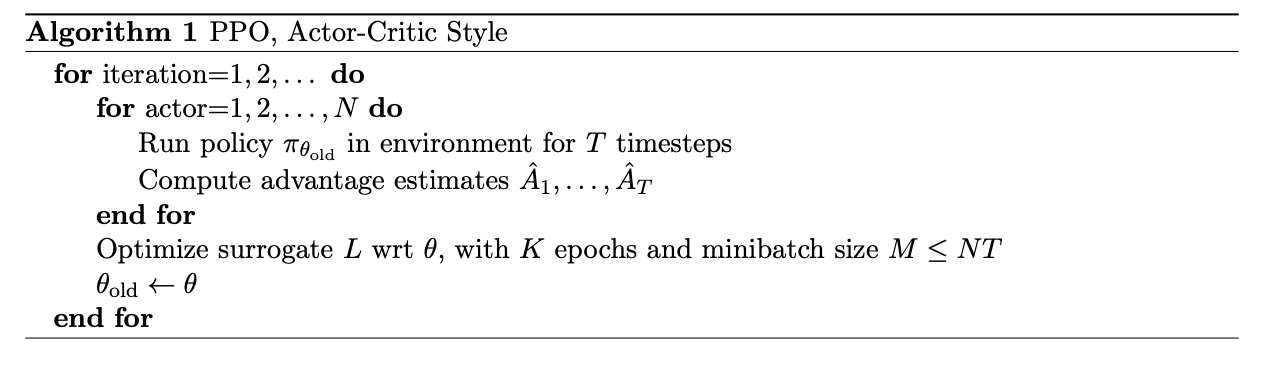
\includegraphics[width=0.95\textwidth]{images/ppo-algo.png}
%     \caption{Agent Inputs}
%     \label{fig:rl}
% \end{figure}


\begin{algorithm}[H]
\caption{Proximal Policy Optimization (PPO)}\label{alg:ppo}
\begin{algorithmic}
\For {iteration = 1,2,\ldots}
\For {actor = 1,2,\ldots,N}
\State Run policy ${\pi_{\theta}}_{old}$ in the environment for T timesteps
\State Compute advantage estimates $\hat{A_{1}}$,\ldots,$\hat{A_{T}}$
\EndFor
\State Optimize surroage $L$ wrt $\theta$, with K epochs and minibatch size $M \leq NT$\\
\State $\theta_{old} \gets \theta$
\EndFor
\end{algorithmic}
\end{algorithm}


\section{AGENT INPUTS} \label{ch4inp}

The agent in our environment is the Car(1) itself. The car makes decisions regarding acceleration deceleration and steering angle based on the inputs that it receives. The two major types of inputs that the agent perceives from the environment are the current speed and the Ray Perception Senor data(4) from the sensors placed on the car. The Ray Perception inputs inform the car of the distance of the object, what kind of object it is and also the angle from the car at which the object is located. For example, the object could be a Checkpoint(2) or a SideWall(3). The car makes use of this information to decide when to accelerate, brake, or turn.

\begin{figure}[H]
    \centering
    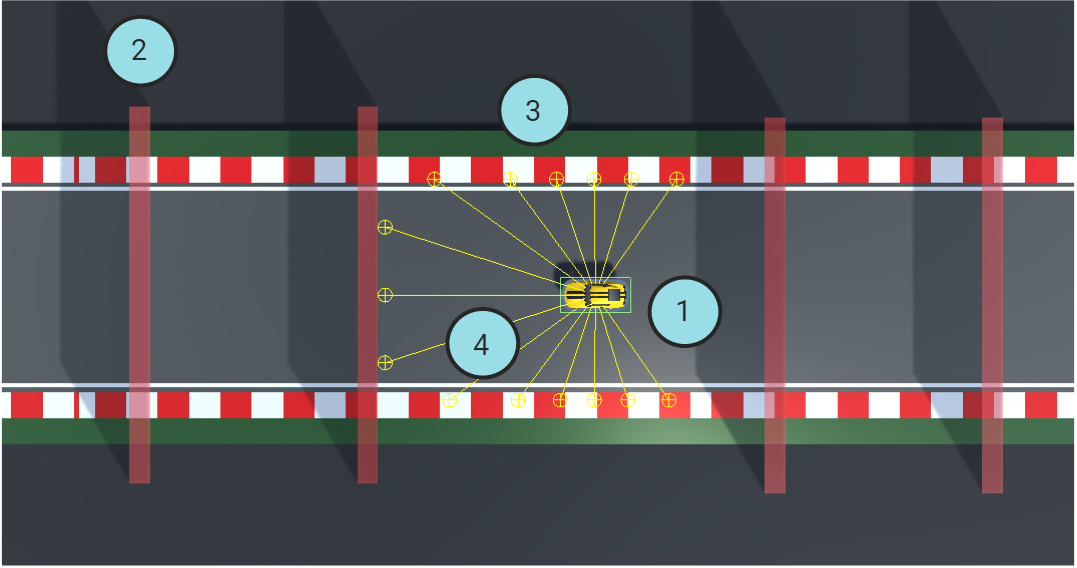
\includegraphics[width=0.75\textwidth]{images/UnityEnv.png}
    \caption{Agent Inputs}
    \label{fig:agent-inputs}
\end{figure}

\section{TRANSFER LEARNING} \label{ch4TL}
Upon training the models on the basic tracks developed using the PPO Algorithm, we then move on to creating complex tracks which we cover in section \ref{ch5} for the purposes of studying the results obtained by using Transfer Learning in our environment. 
\\ We study the performance obtained by TL when the similarity is high (intra basic track) and similarity is lower (basic track - complext track). It is to be noted that the latter is more dissimilar only when compared to the former and that in both cases the source task and the target task have the same task structure, satisfying the requirement to perform TL in RL \cite{TLRLImplement}. We peform these experiments to understand the difficulties associated with using TL in RL to leverage learned representation. 
\\To measure the performance of TL in RL in our environment, we measure the cumulative reward obtained at the end of fixed amount of steps on the target task and compare it with the cumulative reward obtained by training for the same number of steps on the target task with no prior knowledge. We also monitor the variance in  episode length as it is an indicator of the stability of the agent on the track.


\section{ADVERSARIAL  TRAINING} \label{ch4AT}
Finally, we perform Adversarial Attack and Adversarial Training in our environment using noise based attacks on the observations(\ref{at-obs}) and on the action space (\ref{at-action}).
\subsection{Attack on Observation} \label{at-obs}
The observations perceived by the agent are the current speed of the car and the distance and angle at which the checkpoints and walls of the track are located at. For the purposes of attacking the observation space, we add noise to the checkpoint positioning resulting in sub-optimal checkpoint orientation on track. Upon passing through a `attacked checkpoint', we attack the successive checkpoint and finally all checkpoints are reset at the time of lap completion.
\begin{algorithm}[H]
\caption{Adversarial Attack on Checkpoints}\label{alg:cap}
\begin{algorithmic}
\Require checkpointAtttackFlag = True
\State checkpointList[] $\gets$ track.getCheckpointList()
\State nextCheckpoint = 0
\While{lapCompleted = False}
\State $X_{disp} \gets$ Random.RandInt(-4, 4)
\State $Y_{disp} \gets$ Random.RandInt(-4, 4)
\State checkpointList[nextCheckpoint].position += ($X_{disp}$, $Y_{disp})$\\
\State nextCheckpoint = (nextCheckpoint + 1) \% totalCheckpoints\\
\If{nextCheckpoint = 0} \Comment{All checkpoints passed}
\State lapCompleted $\gets$ True
\State reset positions of all checkpoints
\EndIf
\EndWhile
\end{algorithmic}
\end{algorithm}

\subsection{Attack on Action Space} \label{at-action}
In this attack, we randomly pick actions ignoring the output provided by the policy of the agent during a fraction of time steps determined by a parameter called \textit{actionAdversaryThreshold}.

\begin{algorithm}[H]
\caption{Adversarial Attack on Actions}\label{alg:cap}
\begin{algorithmic}
\Require actionAdversaryThreshold $\geq$ 0, policy $\pi$
\State action $\gets \pi$.getAction() 
\State forward = action[0]
\State turn = action[1]
\If{Random.Rand() $\geq$ actionAdversaryThreshold} 
\State $forward \gets$ Random.RandInt(-1, 2)
\State $turn \gets$ Random.RandInt(-1, 2)
\EndIf
\State car.forward = forward
\State car.turn = turn
\end{algorithmic}
\end{algorithm}


We perform experiments and train agents on all the basic and complex tracks using both the attacks as  a precursor and repeat the experiments performed for TL in \ref{ch4TL} and study the performance of TL obtained using AT as a precursor and in the absence of AT.

